%        File: arfc-beamer.tex
%     Created: Sun May 5 10:00 PM 2013 C


%\documentclass[11pt,handout]{beamer}
\documentclass[9pt]{beamer}
\usetheme[white]{Illinois}
%\title[short title]{long title}
\title[Research Summary]{Research Activities in the ARFC Group}
%\subtitle[short subtitle]{long subtitle}
\subtitle[Brief Summary]{A Brief Summary}
%\author[short name]{long name}
\author[ARFC]{Advanced Reactors and Fuel Cycles Group}
%\date[short date]{long date}
\date[09.05.2019]{September 5, 2019}
%\institution[short name]{long name}
\institute[UIUC]{University of Illinois at Urbana-Champaign}

%\usepackage{bbding}
\usepackage{amsfonts}
\usepackage{amsmath}
\usepackage{xspace}
\usepackage{graphicx}
\usepackage{subfigure}
\usepackage{booktabs} % nice rules for tables
\usepackage{microtype} % if using PDF
\usepackage{bigints}
\usepackage{minted}
\usepackage[absolute,overlay]{textpos}
\usepackage{tikz}
\usetikzlibrary{positioning, arrows, decorations, shapes}
\usetikzlibrary{shapes.geometric,arrows}
\definecolor{illiniblue}{HTML}{B1C6E2}
\tikzstyle{bblock} = [rectangle, draw, fill=illiniblue, 
text width=10em, text centered, rounded corners, minimum height=4em]
\tikzstyle{sbblock} = [rectangle, draw, fill=illiniblue, 
text width=7em, text centered, rounded corners, minimum height=4em]
\tikzstyle{arrow} = [thick,->,>=stealth]

\newcommand{\units}[1] {\:\text{#1}}%
\newcommand{\SN}{S$_N$}%{S$_\text{N}$}%{$S_N$}%
\DeclareMathOperator{\erf}{erf}
%I need some complimentary error funcitons... 
\DeclareMathOperator{\erfc}{erfc}
%Those icons in the references are terrible looking
\setbeamertemplate{bibliography item}[text]

%%%% Acronym support

\usepackage[acronym,toc]{glossaries}
\include{acros}

\makeglossaries

%try to get rid of header on title page\dots
\makeatletter
    \newenvironment{withoutheadline}{
        \setbeamertemplate{headline}[default]
        \def\beamer@entrycode{\vspace*{-\headheight}}
    }{}
\makeatother

\makeatother
\setbeamertemplate{footline}
{
  \leavevmode%
  \hbox{%
    \rightline{\insertframenumber{} / \inserttotalframenumber\hspace*{1ex}}
  }%
  \vskip0pt%
}
\makeatletter
\begin{document}
%%%%%%%%%%%%%%%%%%%%%%%%%%%%%%%%%%%%%%%%%%%%%%%%%%%%%%%%%%%%%
%% From uw-beamer Here's a handy bit of code to place at 
%% the beginning of your presentation (after \begin{document}):
\newcommand*{\alphabet}{ABCDEFGHIJKLMNOPQRSTUVWXYZabcdefghijklmnopqrstuvwxyz}
\newlength{\highlightheight}
\newlength{\highlightdepth}
\newlength{\highlightmargin}
\setlength{\highlightmargin}{2pt}
\settoheight{\highlightheight}{\alphabet}
\settodepth{\highlightdepth}{\alphabet}
\addtolength{\highlightheight}{\highlightmargin}
\addtolength{\highlightdepth}{\highlightmargin}
\addtolength{\highlightheight}{\highlightdepth}
\newcommand*{\Highlight}{\rlap{\textcolor{HighlightBackground}{\rule[-\highlightdepth]{\linewidth}{\highlightheight}}}}
%%%%%%%%%%%%%%%%%%%%%%%%%%%%%%%%%%%%%%%%%%%%%%%%%%%%%%%%%%%%%
%%--------------------------------%%
\begin{withoutheadline}
\frame{
  \titlepage
}
\end{withoutheadline}

%%--------------------------------%%
\AtBeginSection[]{
\begin{frame}
  \frametitle{Outline}
  \tableofcontents[currentsection]
\end{frame}
}

\section{Software}
\begin{frame}
\frametitle{Cyclus}
\begin{block}{What is Cyclus?}
	Cyclus is a modular agent based fuel cycle simulator for tracking commodity transactions
	between facilities.
\end{block}
\begin{figure}
	\centering
	\includegraphics[width=0.7\linewidth]{./images/lanl-fuel-cycle.png}
	\label{fig:fuelcycle}
\end{figure}
\end{frame}

\begin{frame}
\frametitle{Why Cyclus?}
Cyclus allows the construction of specific scenarios through the addition of archetypes. These archetypes are
modular and the transactions can be tracked.
	\begin{figure}
		\centering
		\includegraphics[width=0.9\linewidth]{./images/diversion1}
		\caption{Material transactions within Cyclus.}
		\label{fig:transactions}
	\end{figure}
\end{frame}
\begin{frame}
	\frametitle{Moltres}
		\begin{itemize}
			\item Moltres is an application code built on the \gls{MOOSE}
			framework, for the simulation of \glspl{MSR}
			\item MOOSE is an open source finite element framework that
			relies on libMesh and PETSc for advanced meshing and PDE
			solver capabilities
			\item Moltres can run transient, fully implicit coupled
			neutronics/thermal-hydraulics simulations of \glspl{MSR}
			\begin{itemize}
				\item Multi-group neutron diffusion (arbitrary groups)
				\item Delayed neutron precursor advection
				\item Incompressible Navier-Stokes for temperature
				advection-diffusion
				\item 2D axisymmetric or 3D modeling
			\end{itemize}
		\end{itemize}
%		\begin{figure}
%			\centering
%			\includegraphics[width=.9\textwidth]{./images/msre}
%		\end{figure}
\end{frame}

\begin{frame}
	\frametitle{Moltres}
	\textbf{MSRE (2D axisymmetric model)}
	\begin{figure}
		\centering
		\includegraphics[width=.9\textwidth]{./images/msre}
		\caption{Group 1 flux, temperature, and longest-lived
		precursor distributions of a 2D axisymmetric MSRE model}
	\end{figure}
\end{frame}
\begin{frame}
\frametitle{SaltProc flowchart}
\vspace{-2mm}
\begin{figure}[ht!] % replace 't' with 'b' to \centering
	\centering
	\includegraphics[width=1.05\textwidth]{./images/saltproc_flowchart.pdf}
	\caption{Tentative generic flowchart for SaltProc v1.0 python package.}
\end{figure}

\end{frame}
\input{annsa}
\documentclass{beamer}
% \usetheme{Illinois}
\usecolortheme{IllinoisWhite}

\title{Machine Learning Applications in Nuclear Engineering}
\author{Sam Dotson}
\institute{University of Illinois at Urbana-Champaign}
\date{2019}

\begin{document}
\frame{\titlepage}
	\begin{frame}
		\frametitle{Table of Contents}
		\tableofcontents
	\end{frame}

	\section{ANNSA}

	\begin{frame}
		\frametitle{\texttt{ANNSA}}
		``$\textbf{A}$rtificial $\textbf{N}$eural $\textbf{N}$etworks for $\textbf{S}$pectroscopic $\textbf{A}$nalysis"\\
		\begin{enumerate}
			\item Isotopics
			\item Nuclear Verification
			\item National Security 
			\item Machine Learning
		\end{enumerate}
	\end{frame}	

	\begin{frame}
		
	\end{frame}

	\section{CAIRO}

	\begin{frame}
		\frametitle{\texttt{CAIRO}}
		``$\textbf{C}$omputerized $\textbf{A}$rtificially $\textbf{I}$ntelligent $\textbf{R}$eactor $\textbf{O}$perator"\\
		\begin{enumerate}
			\item Nuclear Power
			\item Reactor Controls
			\item Control Room Simulation
			\item Artificial Intelligence
		\end{enumerate}
	\end{frame}
\end{document}
\section{Advanced Reactors}
\begin{frame}
	\frametitle{Sun Myung Park: Coupled neutronics/thermal-hydraulics analysis}
		\begin{columns}
		\column[t]{6cm}
		My current research interests:
		\begin{block}{Moltres}
			\begin{itemize}
				\item Developing and improving capabilities in Moltres \\
				\item Currently working on
				implementing the k-$\epsilon$ turbulence model in Moltres.
			\end{itemize}
		\end{block}
		\begin{block}{\gls{MSFR}}
			\begin{itemize}
			\item Performing safety analyses of the \gls{MSFR} for various
			accident transients using Moltres with the k-$\epsilon$ model to
			include turbulence effects
			\end{itemize}
		\end{block}
		\column[t]{4cm}
		\begin{figure}[htbp!]
			\begin{center}
				\includegraphics[height=3cm]{./images/msfr}
			\end{center}
			\caption{Schematic diagram of the \gls{MSFR}}
			\label{fig:msfr}
		\end{figure}
		\end{columns}
\end{frame}

\begin{frame}
	\frametitle{Sun Myung Park}
		\begin{columns}
			\column[t]{.5\textwidth}
			\begin{figure}[htbp!]
				\centering
				\includegraphics[height=2.8cm]{./images/mesh}
      			\includegraphics[height=2.8cm]{./images/loscaheat}
    			\caption{\scriptsize Clockwise from top left: MSFR 2D
    			axisymmetric mesh, steady state fuel temperature distribution,
    			relative power during a loss of heat sink scenario.}
			\end{figure}
			\vspace{.1cm}
			\column[t]{.5\textwidth}
			\begin{figure}
				\centering
				\includegraphics[width=.9\textwidth]{./images/ins-flow}
				\caption{\footnotesize Velocity distribution produced from the
				incompressible Navier-Stokes equations}
			\end{figure}
		\end{columns}
\end{frame}
\begin{frame}
	\frametitle{Ansh - Energy Analysis for Decarbonization in Japan}
	% a comment
  \begin{figure}[htbp!]
    \begin{center}
      \includegraphics[scale=0.5]{./images/conv_nuc_elc}
    \end{center}
          \caption{Electricity generation in Japan without constraints on nuclear energy. Scenario simulated using TIMES.}
    \label{s1e}
  \end{figure}

\end{frame}

\begin{frame}
	\frametitle{Ansh - Recirculation zones in MSRE}
	% a comment
  \begin{figure}[htbp!]
    \begin{center}
      \includegraphics[scale=0.25]{./images/msre-flat}
    \end{center}
          \caption{LES simulation of MSRE channel without pyramid stringer using Nek5000.}
    \label{s1e}
  \end{figure}

\end{frame}

\begin{frame}
\frametitle{Transatomic Power (TAP) concept high-fidelity Serpent model}
	  \begin{textblock*}{12.25cm}(0.25cm,1.8cm) % {block width} (coords)
\begin{figure}[htp!] % replace 't' with 'b' to 
	\includegraphics[width=\textwidth]{./images/tap_model.png}
	\caption{An $XY$ (left) and $XZ$ (right) section of the TAP model. 
	The violet color represents zirconium hydride, and the yellow represents 
	fuel salt (reproduced from Rykhlevskii \& Huff, Milestone 2.1 Report, 
	2019).}
\end{figure}
	  \end{textblock*}
\end{frame}


\begin{frame}
\frametitle{Depletion simulation results for TAP with various feeds}       
\begin{textblock*}{12.6cm}(0.1cm,2.2cm) % {block width} (coords)
	\begin{figure}[htp!] % replace 't' with 'b' to 
		\begin{minipage}[b]{0.48\textwidth}
			\includegraphics[width=\linewidth]{./images/keff_3.png}
		\end{minipage}
			\hspace{-2mm}
		\begin{minipage}[b]{0.48\textwidth}
			\includegraphics[width=\linewidth]{./images/keff_zoomed_2.png}
		\end{minipage}
		\caption{Effective multiplication factor dynamics for full-core
		TAP model for different fueling scenarios over a 13-year reactor 
		operation (left) and for the time interval from 367 to 471 days after 
		startup (right). Confidence interval $\pm\sigma=28pcm$ is shaded.}
	\end{figure}
\end{textblock*}
\end{frame}


\begin{frame}
\frametitle{Fuel salt composition evolution during the TAP operation}
\begin{textblock*}{12.25cm}(0.25cm,2cm) % {block width} (coords)
	\begin{figure}[htp!] % replace 't' with 'b' to 
		\centering
				\vspace{-3mm}
		\includegraphics[width=0.72\textwidth]{../images/u_pu_mass.png}
		\caption{Mass of major nuclides during 13 years of reactor operation 
		with 19.79\% low-enriched uranium feed.}
	\end{figure}
\end{textblock*}
\end{frame}
\begin{frame}
\frametitle{Microreactors: Motivation}
\begin{columns}
  \column[t]{5cm}
  Microreactors can fulfill energy needs in special use cases, or in
  areas with a greater population.
  \column[t]{5cm}
    \begin{figure}[htbp!]
    \begin{center}
    \includegraphics[height=4cm]{./images/mmr-chalk-river}
    \end{center}
    \caption{A Diagram of the proposed MMR for the Chalk River project. \cite{mmr-chalk-river}.}
    \label{fig:kittenfigure}
    \end{figure}

\end{columns}
\end{frame}


\begin{frame}
\frametitle{Siting Considerations for Microreactors}

  \begin{itemize}
    \item Current guidelines based on LWRS
    \item Experience tells us radionuclide release is not as severe as once feared.
  \end{itemize}

  The first step in these revised siting considerations is to determine a source term.

\end{frame}

\begin{frame}
	\frametitle{Roberto Fairhurst: Compressibility in Moltres}
		\begin{columns}
		\column[t]{6cm}

		Compressibility in liquids:
		
            \begin{align}
			\rho (\vec{v}.\nabla)\vec{v} + \nabla p - \rho g \check{j} - \mu \nabla^{2}\vec{v} = 0 \\
			\vec{v}.\nabla\rho+\rho\nabla.\vec{v}=0 \\
			\rho c_{v} (\vec{v}.\nabla)T - \nabla .(k\nabla T) + p (\nabla . \vec{v})= 0 \\
			\rho = \rho_{0} + \frac{\rho_{0}}{K}(p-p_{0}) + \rho_{0}\beta(T-T_{0})
            \end{align}

			\begin{itemize}
				\item Density dependency on pressure and temperature for liquids.
				\item Next, implement it for gasses $p=\rho RT$
			\end{itemize}

		\column[t]{5cm}
		\begin{figure}[htbp!]
			\begin{center}
				\includegraphics[height=2cm]{./images/liquid_compres.png}
			\end{center}
			\caption{Vertical velocity.}
			\label{fig:velocity}
		\end{figure}

		\begin{figure}[htbp!]
			\begin{center}
				\includegraphics[height=2cm]{./images/rho.png}
			\end{center}
			\caption{Density distribution.}
			\label{fig:density}
		\end{figure}

		\end{columns}
\end{frame}
\section{Fuel Cycles}
\begin{frame}
  \frametitle{Diversion Detection with Cyclus}
  	\textbf{Motivation}
        \begin{itemize}
                \item Safeguard by design
                \item Model diversion inside facilities
                \item transition from LWR to SFR
        \end{itemize}
    \textbf{Goals}
    	\begin{itemize}
    		\item Detect diversion using signatures and observables.
    		\item Optimum detector and inspection locations in pyroprocessing
    		\item Characterize detection sensitivities and false positive rates
    	\end{itemize}
  \begin{figure}
    \includegraphics[width=0.7\linewidth]{./images/westphal-diversion}
    \caption{Operator vs nefarious diversion.}
    \label{fig:diversion}
  \end{figure}
\end{frame}

\begin{frame}
	\frametitle{PyRe Archetype}
	\begin{columns}
		\column[t]{6cm}
		\begin{itemize}
			\item Facility containing multiple sub-processes:
			\begin{itemize}
				\item Separately handled.
				\item Independent transactions, possibility of diversion.
			\end{itemize}
			\item Operation setting impact efficiency.
			\item Generic facility:
			\begin{itemize}
				\item Multiple types of pyro plants.
				\item LWR vs SFR.
			\end{itemize}
		\end{itemize}
		\begin{block}{Diversion Detection}
			Material transactions are no longer a reliable method. Instead we use
			signatures and observables:
			\begin{itemize}
				\item Temperature, power draw, etc.
			\end{itemize}
			A Cumulative Sum change algorithm is used to detect any significant changes.
		\end{block}
		\column[t]{5cm}
		\begin{figure}
			\includegraphics[width=\linewidth]{./images/westphal-pyre.pdf}
			\caption{PyRe flow diagram for LWR waste configuration.}
			\label{fig:pyre}
		\end{figure}
	\end{columns}
\end{frame}
\begin{frame}
    \frametitle{Sensitivity Analysis with Fuel Cycle Codes}
    \textbf{Motivation for conducting sensitivity analysis}
    \\

    A transition scenario is simulated to predict the 
    future, however when implemented in the real world, 
    it will deviate from the optimal scenario. 
    Therefore, sensitivity analysis studies is necessary to 
    determine how variation in different parameters will impact 
    the progression and final state of the transition scenario. 
    \\

    \textbf{Method}

    Couple fuel cycle codes, \textsc{Cyclus}/DYMOND, 
    with Dakota \cite{eldred_dakota_2010} (sensitivity analysis, 
    optimization, and uncertainty quantification framework).  

    \begin{figure}[]
        \centering
        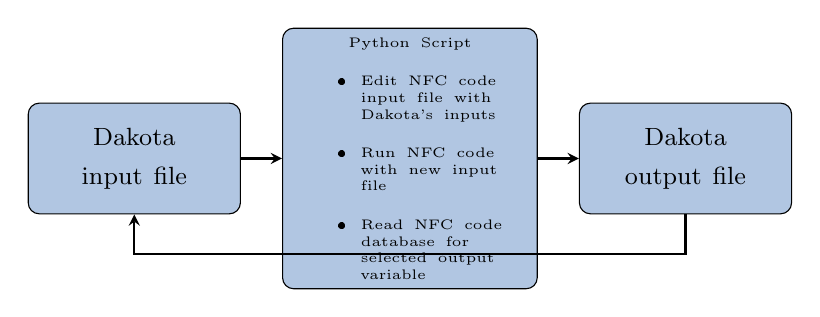
\begin{tikzpicture}[node distance=2.5cm]
            \tikzstyle{every node}=[font=\large]
            \node (one) [sbblock]{\small Dakota input file};
        \node (two) [bblock, right of=one, xshift = 1cm, text width=3cm]{\tiny Python Script\begin{itemize}
            \item Edit NFC code input file with Dakota's inputs 
            \item Run NFC code with new input file 
            \item Read NFC code database for selected output variable
        \end{itemize}};
        \node  (three) [sbblock, xshift = 1cm, right of=two]{\small Dakota output file};
            
            \draw [arrow] (one) -- (two);
            \draw [arrow] (two) -- (three);
            %\draw [arrow] (three) -- (one);
            %\draw [arrow] (All) -- node[anchor=west] {yes} (End);
            %draw [arrow] (All) -- ([shift={(-3.9cm,0.7cm)}]All.south west)-- node[anchor=east] {no} ([shift={(-3.9cm,-0.85cm)}]Predict.north west)--(Predict);
            \draw [arrow] (three) |-([shift={(0cm,-0.5cm)}]three.south west)-- ([shift={(0cm,-0.5cm)}]one.south east)-|(one);
        \end{tikzpicture}
        \caption{Depiction of coupling of Dakota and NFC code}
        \label{fig:dakota-NFC-flow}
    \end{figure}

\end{frame}
\begin{frame}
    \frametitle{Demand-Driven Cycamore Archetypes Project (NEUP-FY16-10512) }
          \begin{columns}
                  \column[t]{5cm}
                  \textbf{Goal of DDCA Project}
                  \\
                  \vspace{0.1cm} 
                  \begin{itemize}
                      \item Design a \textsc{Cyclus} institution 
                      that will
                      automatically deploy supporting fuel 
                      cycle facilities and reactor 
                      facilities for a user-specified 
                      power demand.
                      \item Demonstrate setting up of 
                      transition scenarios 
                      with undersupply of power. 
                  \end{itemize}
                  \textbf{Progress}
                  \vspace{0.1cm} 
                  \begin{itemize}
                    \item Created \textsc{Cyclus} institution: 
                    \texttt{deploy}
                    \item Set up transition scenarios 
                    (EG01-23/24/29/30 \cite{wigeland_nuclear_2014}) 
                    using \texttt{deploy}
                  \end{itemize}
                  \column[t]{5cm}
          \begin{figure}[htbp!]
          \begin{center}
        \includegraphics[height=5.5cm]{./images/d3ploy-flow}
      \end{center}
            \caption{\texttt{d3ploy} logic flow \cite{chee_demonstration_2019}}
      \label{fig:d3ploy-flow}
    \end{figure}
          \end{columns}
  \end{frame}

\begin{frame}
	\frametitle{Roberto Fairhurst: Transition Scenarios}
		\begin{columns}
		\column[t]{6cm}
		Current research interests:
		\begin{block}{D3ploy}
			\begin{itemize}
				\item Obtaining results for all the scenarios.
				\item Putting together final report.
			\end{itemize}
		\end{block}

        \begin{figure}[htbp!]
     	\begin{center}
				\includegraphics[height=3cm]{./images/eg23-power-poly}
			\end{center}
			\caption{Demand and supply of power for scenario eg01-eg23 using polynomial fit.}
			\label{fig:eg23-power}
	    \end{figure}

		\column[t]{4cm}
		\begin{figure}[htbp!]
			\begin{center}
				\includegraphics[height=3cm]{./images/eg23-frfuel}
			\end{center}
			\caption{Demand and supply of FR fuel for scenario eg01-eg23 using polynomial fit.}
			\label{fig:eg23-frfuel}
		\end{figure}
		\end{columns}
\end{frame}

\section{Acknowledgments}
\begin{frame}
  \frametitle{Acknowledgments}
        Acknowledgements should include both people who helped and funding 
        streams. If you are funded by an NEUP grant, that number usually goes 
        here. .
\end{frame}

%%--------------------------------%%
%%--------------------------------%%
\begin{frame}[allowframebreaks]
  \frametitle{References}
  \bibliographystyle{plain}
  {\footnotesize \bibliography{2019-09-05-group.bib} }
\end{frame}

%%--------------------------------%%

% Examples 
% ARFC Team: Some good examples of how to use beamer are in this file.
% You can use this to guide the preparation of slides.
% ARFC Team: Some good examples of how to use beamer are in this file.
% You can use this to guide the preparation of slides.

\begin{frame}
  \frametitle{Columns}
  % a comment
        \begin{columns}
                \column[t]{5cm}
                Sometimes things need to be put side by side, in two nice
                looking columns.

                Maybe one column involves a quotation.

                \begin{quote}
                        Explicit is better than implicit. -- The Zen of Python
                \end{quote}


                And, also, perhaps, a logo.
                \begin{center}
                        \includegraphics[height=0.2\textheight]{./images/arfc-logo}
                \end{center}
                \column[t]{5cm}
        \begin{figure}[htbp!]
        \begin{center}
      \includegraphics[height=4cm]{./images/kitten}
    \end{center}
          \caption{A caption describing the image. \cite{lastname_firstword_1900}.}
    \label{fig:kittenfigure}
  \end{figure}
        \end{columns}
\end{frame}

\begin{frame}[fragile]
  \frametitle{Some Code}
        I have to use the fragile syntax for code slides.
        \begin{minted}{python}
def meow(volume):
    """Make a demanding noise at the specified volume

    Parameters
    ----------
    volume: int
        The volume of the demand. No relation to importance.

    Returns
    -------
    str
        meow
    """
    o = 'o'*volume
    return 'me'+ o + 'ow'
\end{minted}
\end{frame}
\begin{frame}
  \frametitle{An Image}
  % a comment
  \begin{figure}[htbp!]
    \begin{center}
      \includegraphics[height=4cm]{./images/kitten}
    \end{center}
          \caption{A caption describing the image. \cite{lastname_firstword_1900}.}
    \label{fig:kittenfigure}
  \end{figure}
\end{frame}

\begin{frame}
  \frametitle{A Table}
        Frames (slides) can have ``blocks.''
        \begin{block}{This one is about a cat}
                A cat in a hat.
        \end{block}
        \begin{block}{A cat}
                In a hat.

                \includegraphics[height=0.2\textheight]{./images/catinhat}
        \end{block}

\end{frame}
\begin{frame}
  \frametitle{Cat Math: Part 1}
  % a comment
        \begin{align}
                x &= y
                \intertext{where}
                x &= \mbox{cats}\\
                y &= \mbox{peculiar}
        \end{align}
\end{frame}

\begin{frame}
\frametitle{Cat Math: Part 2}
        Everything in Beamer is just like in \LaTeX.
        Right down to the theorems.
        \begin{theorem}[Pythagoras]
                $ a^2 + b^2 = c^2$
        \end{theorem}
        \begin{corollary}
                $ x + y = y + x  $
        \end{corollary}
        \begin{proof}
                $\omega +\phi = \epsilon $
        \end{proof}

\end{frame}

\begin{frame}
  \frametitle{Blue and Orange are Fierce}
  % a comment
        Those are the Illini Colors. Use them like you see them in Figure
        \ref{fig:fierce}.
  \begin{figure}[htbp!]
    \begin{center}
      \includegraphics[height=4cm]{./images/fierce}
    \end{center}
          \caption{Kristofer Hivju is pretty serious about this color palette \cite{lastname_firstword_1900}.}
    \label{fig:fierce}
  \end{figure}
\end{frame}


\begin{frame}
        \frametitle{Table}
        \input{tab}
\end{frame}





\end{document}

